\documentclass{article}

\usepackage{amsthm}
\usepackage{amsfonts}
\usepackage{amsmath}
\usepackage{amssymb}
\usepackage{fullpage}
\usepackage{graphicx}
\usepackage[usenames]{color}
\usepackage{hyperref}
  \hypersetup{
    colorlinks = true,
    urlcolor = blue,       % color of external links using \href
    linkcolor= blue,       % color of internal links 
    citecolor= blue,       % color of links to bibliography
    filecolor= blue,        % color of file links
    }
    
\usepackage{listings}

\definecolor{dkgreen}{rgb}{0,0.6,0}
\definecolor{gray}{rgb}{0.5,0.5,0.5}
\definecolor{mauve}{rgb}{0.58,0,0.82}
\definecolor{mPurple}{rgb}{0.58,0,0.82}
\definecolor{mGreen}{rgb}{0,0.6,0}
\definecolor{red}{rgb}{1,0,0}

\lstdefinestyle{HaskellStyle}{
  frame=tb,
  language=haskell,
  aboveskip=3mm,
  belowskip=3mm,
  showstringspaces=false,
  columns=flexible,
  basicstyle={\small\ttfamily},
  numbers=none,
  numberstyle=\tiny\color{gray},
  keywordstyle=\color{blue},
  commentstyle=\color{dkgreen},
  stringstyle=\color{mauve},
  breaklines=true,
  breakatwhitespace=true,
  tabsize=3
}

\lstdefinestyle{CStyle}{
  frame=tb,
  language=C,
  aboveskip=3mm,
  belowskip=3mm,
  showstringspaces=false,
  columns=flexible,
  basicstyle={\small\ttfamily},
  numbers=none,
  numberstyle=\tiny\color{gray},
  keywordstyle=\color{blue},
  commentstyle=\color{red},
  stringstyle=\color{mauve},
  breaklines=true,
  breakatwhitespace=true,
  tabsize=3
}

\lstset{frame=tb,
  language=haskell,
  aboveskip=3mm,
  belowskip=3mm,
  showstringspaces=false,
  columns=flexible,
  basicstyle={\small\ttfamily},
  numbers=none,
  numberstyle=\tiny\color{gray},
  keywordstyle=\color{blue},
  commentstyle=\color{dkgreen},
  stringstyle=\color{mauve},
  breaklines=true,
  breakatwhitespace=true,
  tabsize=3
}

\theoremstyle{theorem} 
   \newtheorem{theorem}{Theorem}[section]
   \newtheorem{corollary}[theorem]{Corollary}
   \newtheorem{lemma}[theorem]{Lemma}
   \newtheorem{proposition}[theorem]{Proposition}
\theoremstyle{definition}
   \newtheorem{definition}[theorem]{Definition}
   \newtheorem{example}[theorem]{Example}
\theoremstyle{remark}    
  \newtheorem{remark}[theorem]{Remark}


\title{CPSC-402 Report\\Compiler Construction}
\author{Scott Fitzpatrick  \\ Chapman University}

\date{\today}

\begin{document}

\maketitle

\begin{abstract}

\end{abstract}

\tableofcontents


\section{Introduction}\label{intro}


\section{Homework}\label{homework}

\subsection{Week 1}

\noindent
Exercise 2.2.4: Give DFA's accepting the following languages over the alphabet $\{0,1\}$:

\medskip
b) The set of all strings with three consecutive 0's (not necessarily at the end)

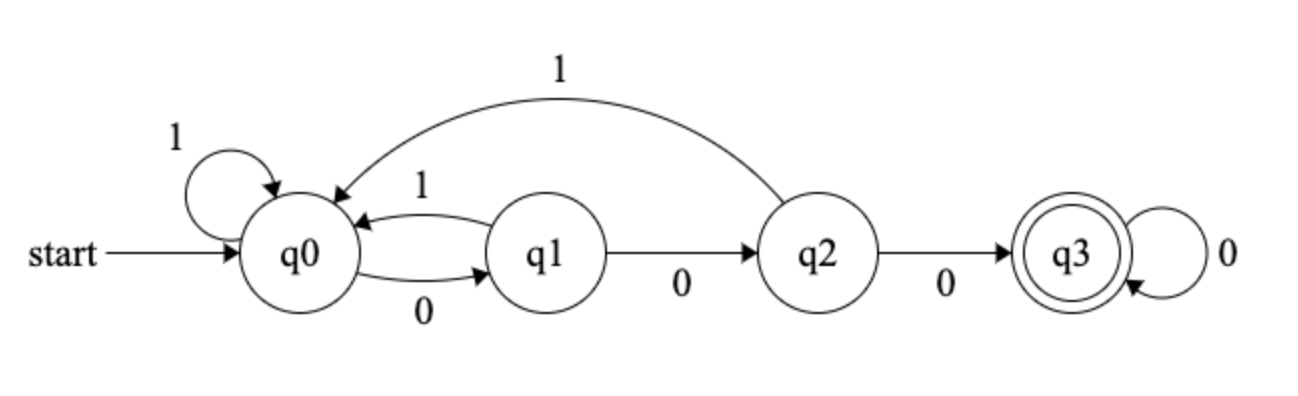
\includegraphics[width=0.75\textwidth]{Images/2.4.4b.png}

\medskip
c) The set of strings with 011 as a substring

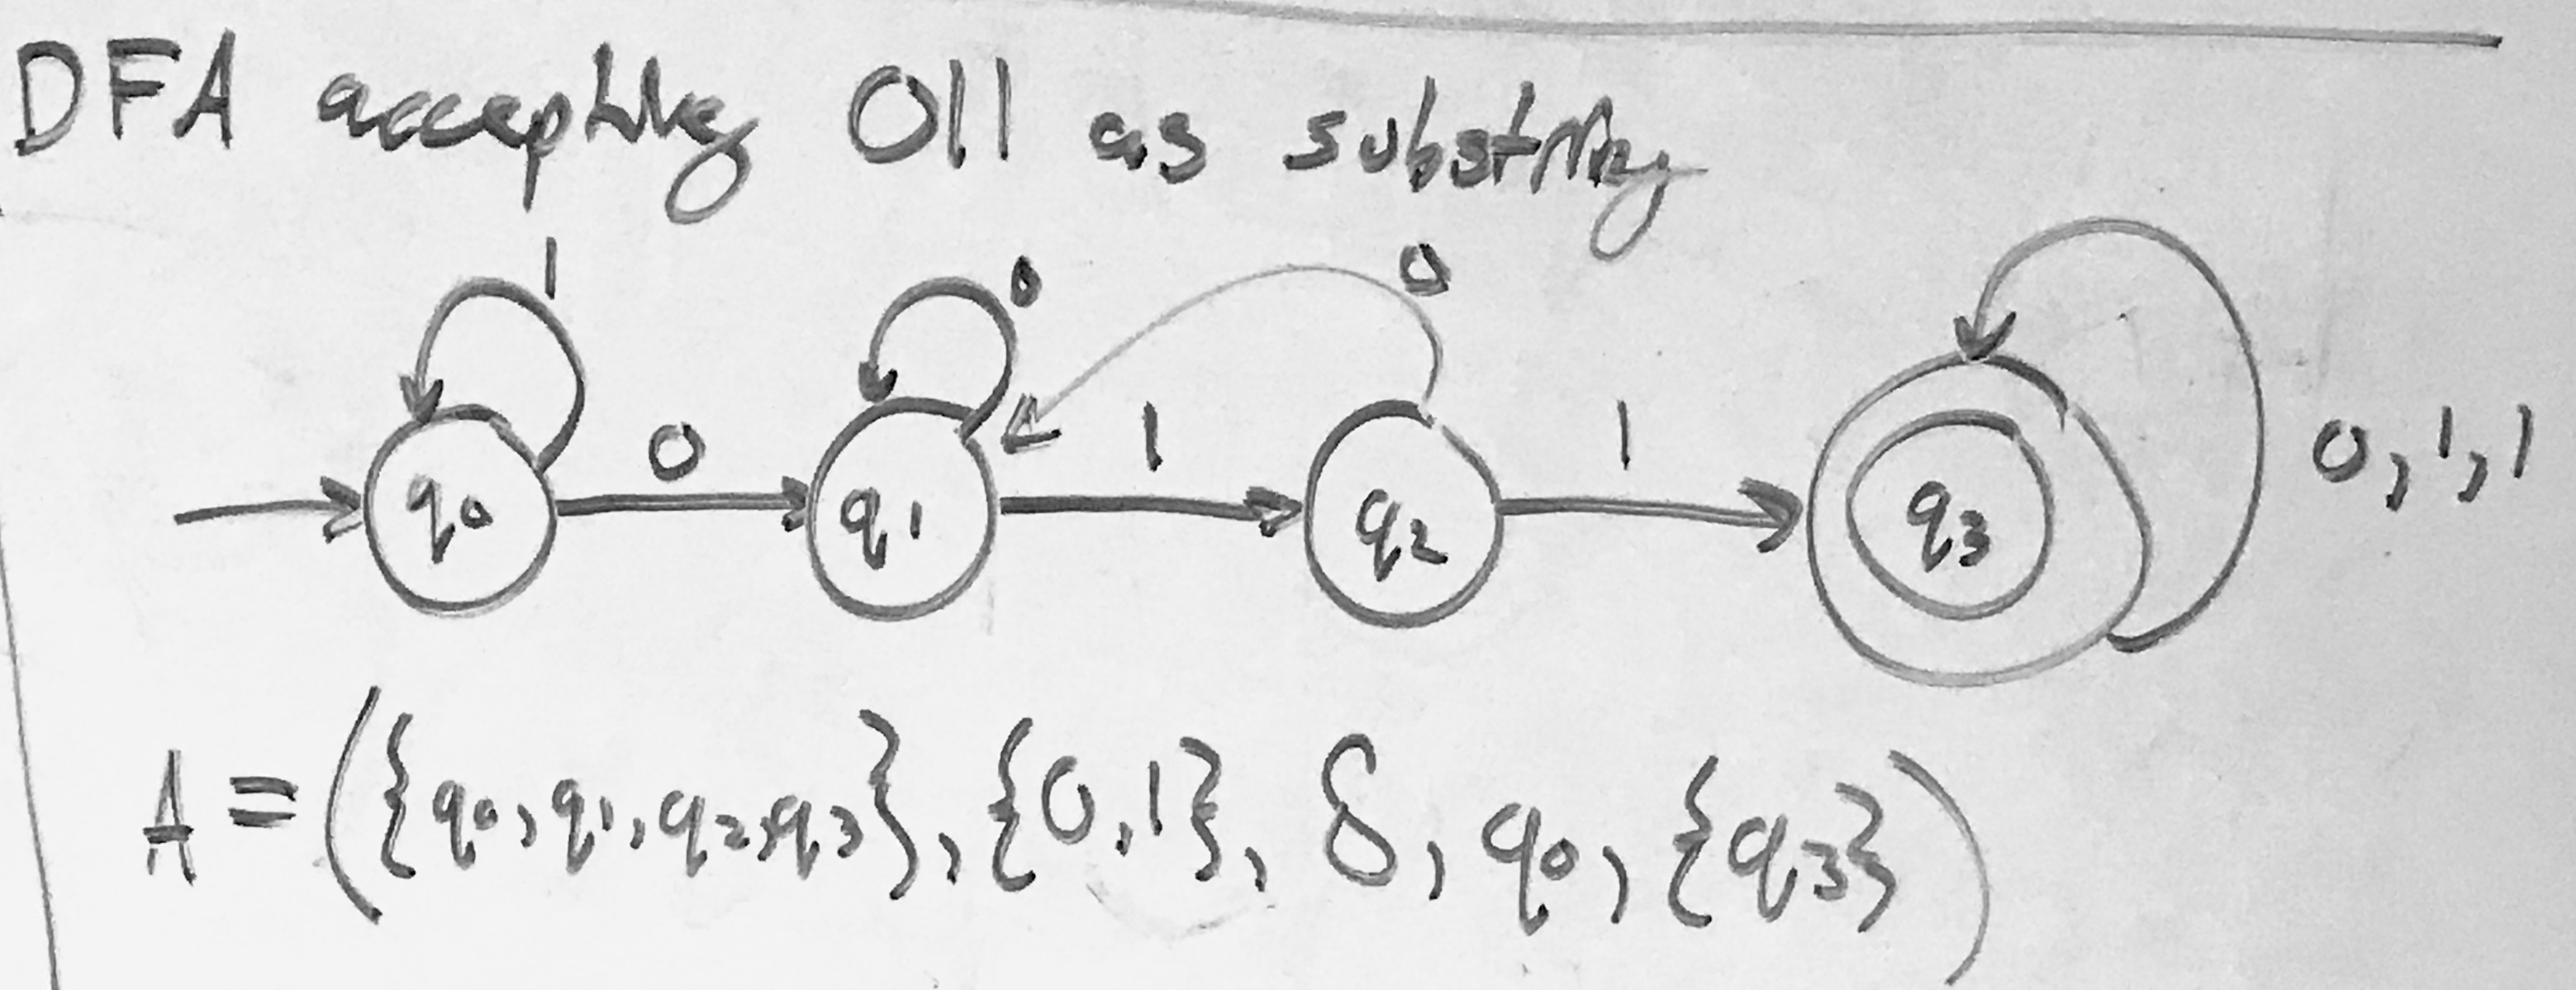
\includegraphics[width=0.75\textwidth]{Images/2.4.4c.png}


\subsection{Week 2}

\noindent
Exercise 2.3.4: a) The set of strings over alphabet $\{0,1,..., 9\}$ such that the final digit has appeared before. b) The set of strings over alphabet $\{0,1,...,9\}$ such that the final digit has not appeared before. c) The set of strings of $0$'s and $1$'s such that there are two $0$'s separated by a number of positions that is a number of $4$. Note that $0$ is an allowable multiple of $4$.

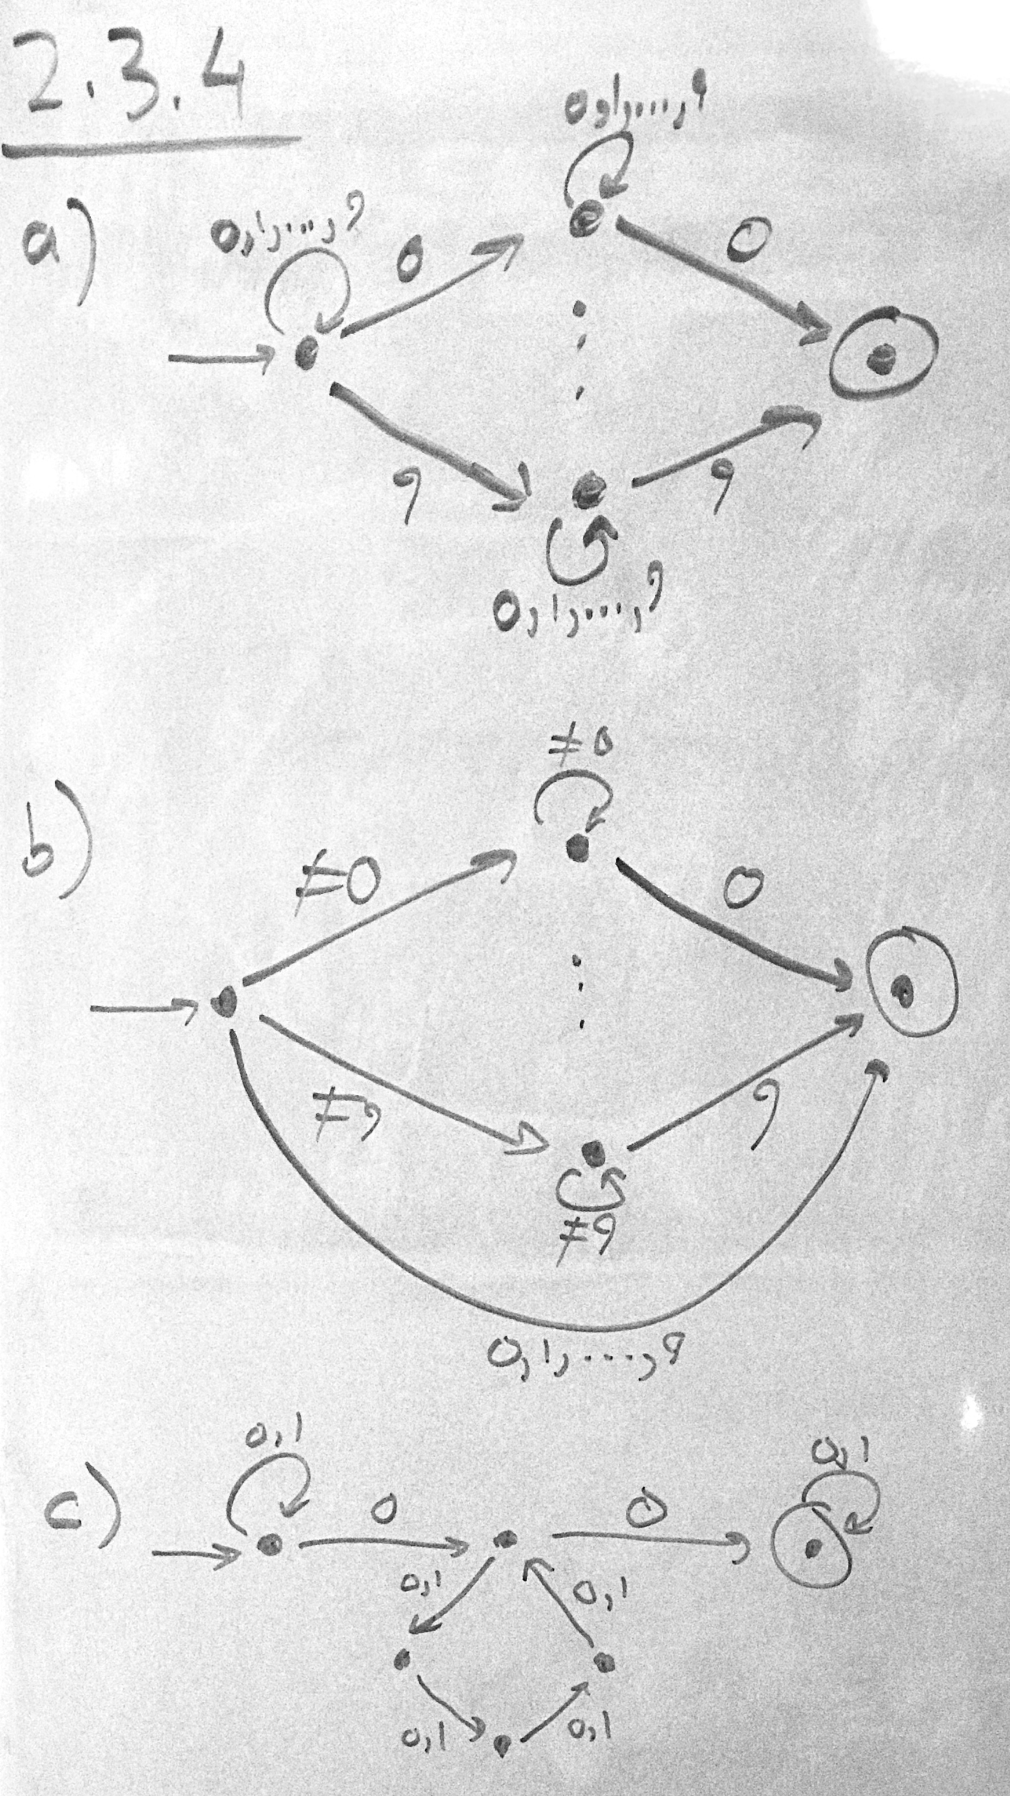
\includegraphics[width=0.55\textwidth]{Images/2.3.4.png}

\medskip\noindent
Exercise 2.5.3: a) The set of strings consisting of zero or more a's followed by zero or more $b$'s, followed by zero or $c$'s. b) The set of strings that consist of either $01$ repeated one or more times or $010$ repeated one or more times. c) The set of strings of $0$'s and $1$'s such that at least one of the last ten positions is a $1$.

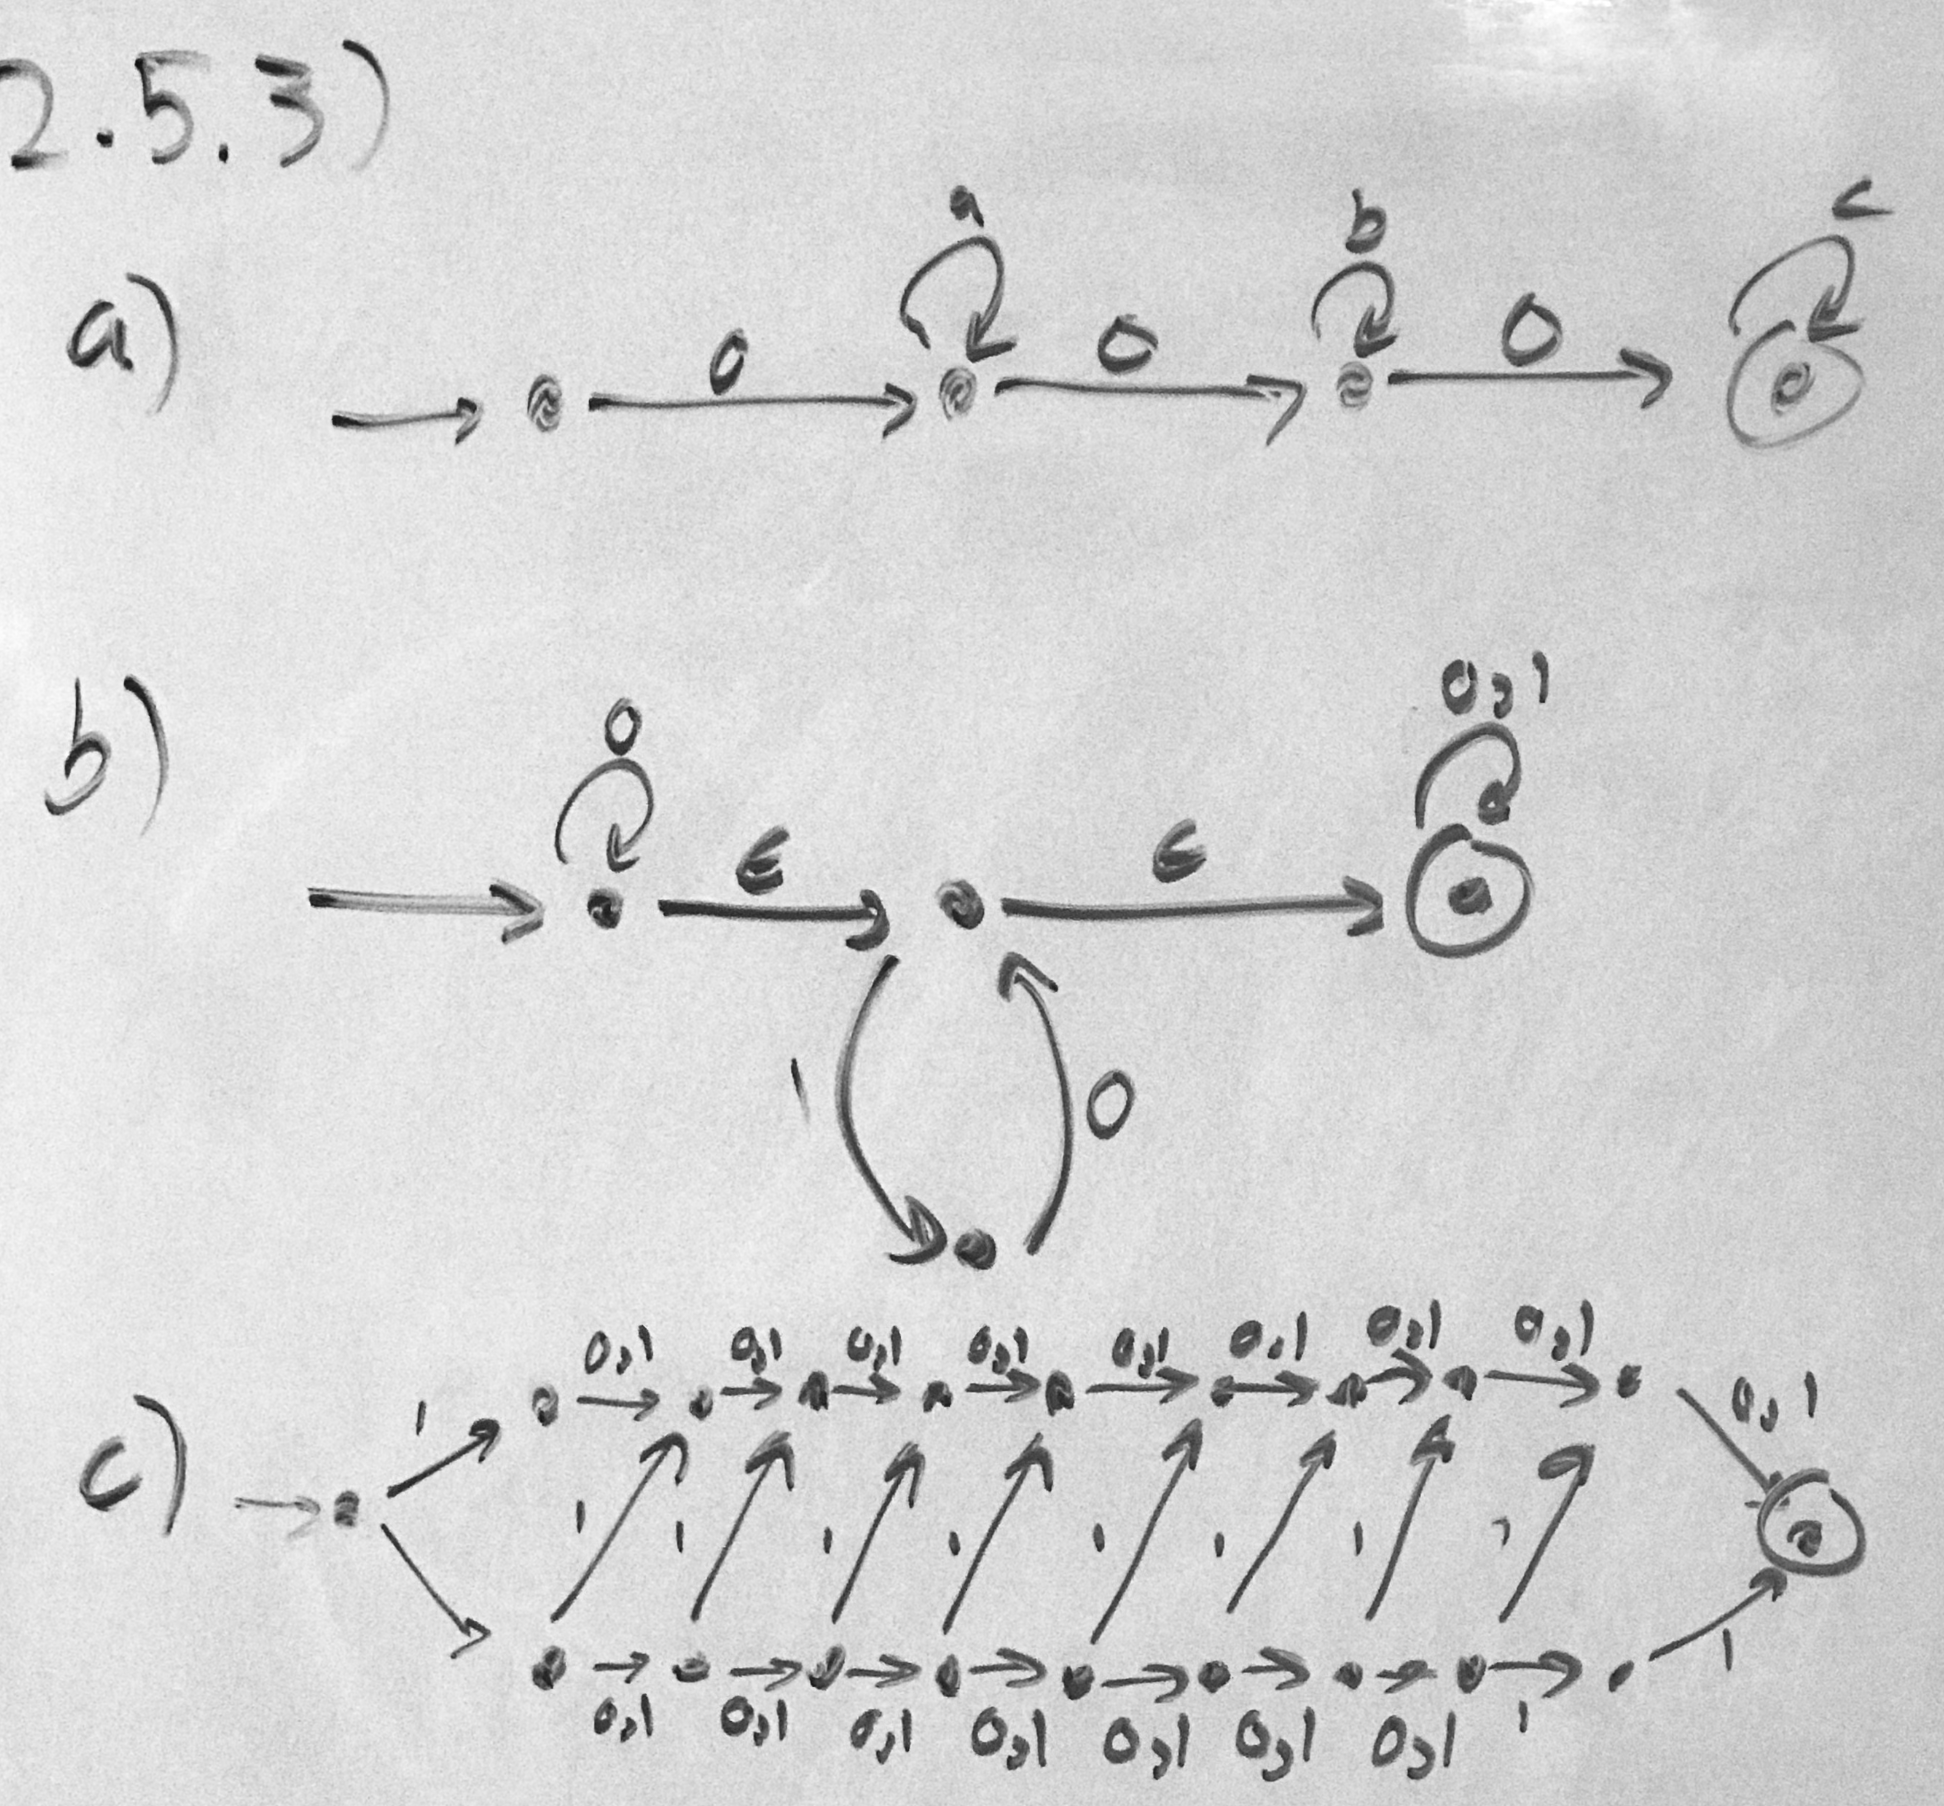
\includegraphics[width=0.75\textwidth]{Images/2.5.3.png}


\subsection{Week 3}

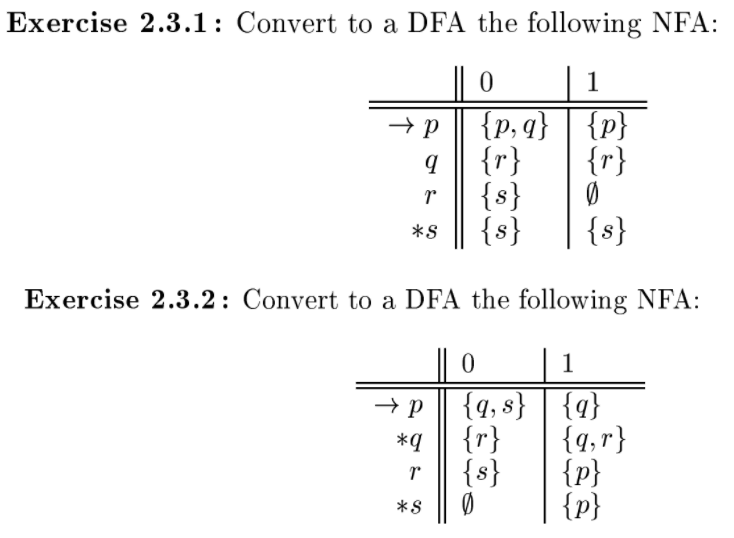
\includegraphics[width=0.65\textwidth]{Images/2.3.1and2.3.2_chart.png}

\noindent
The following DFAs above can be drawn as:

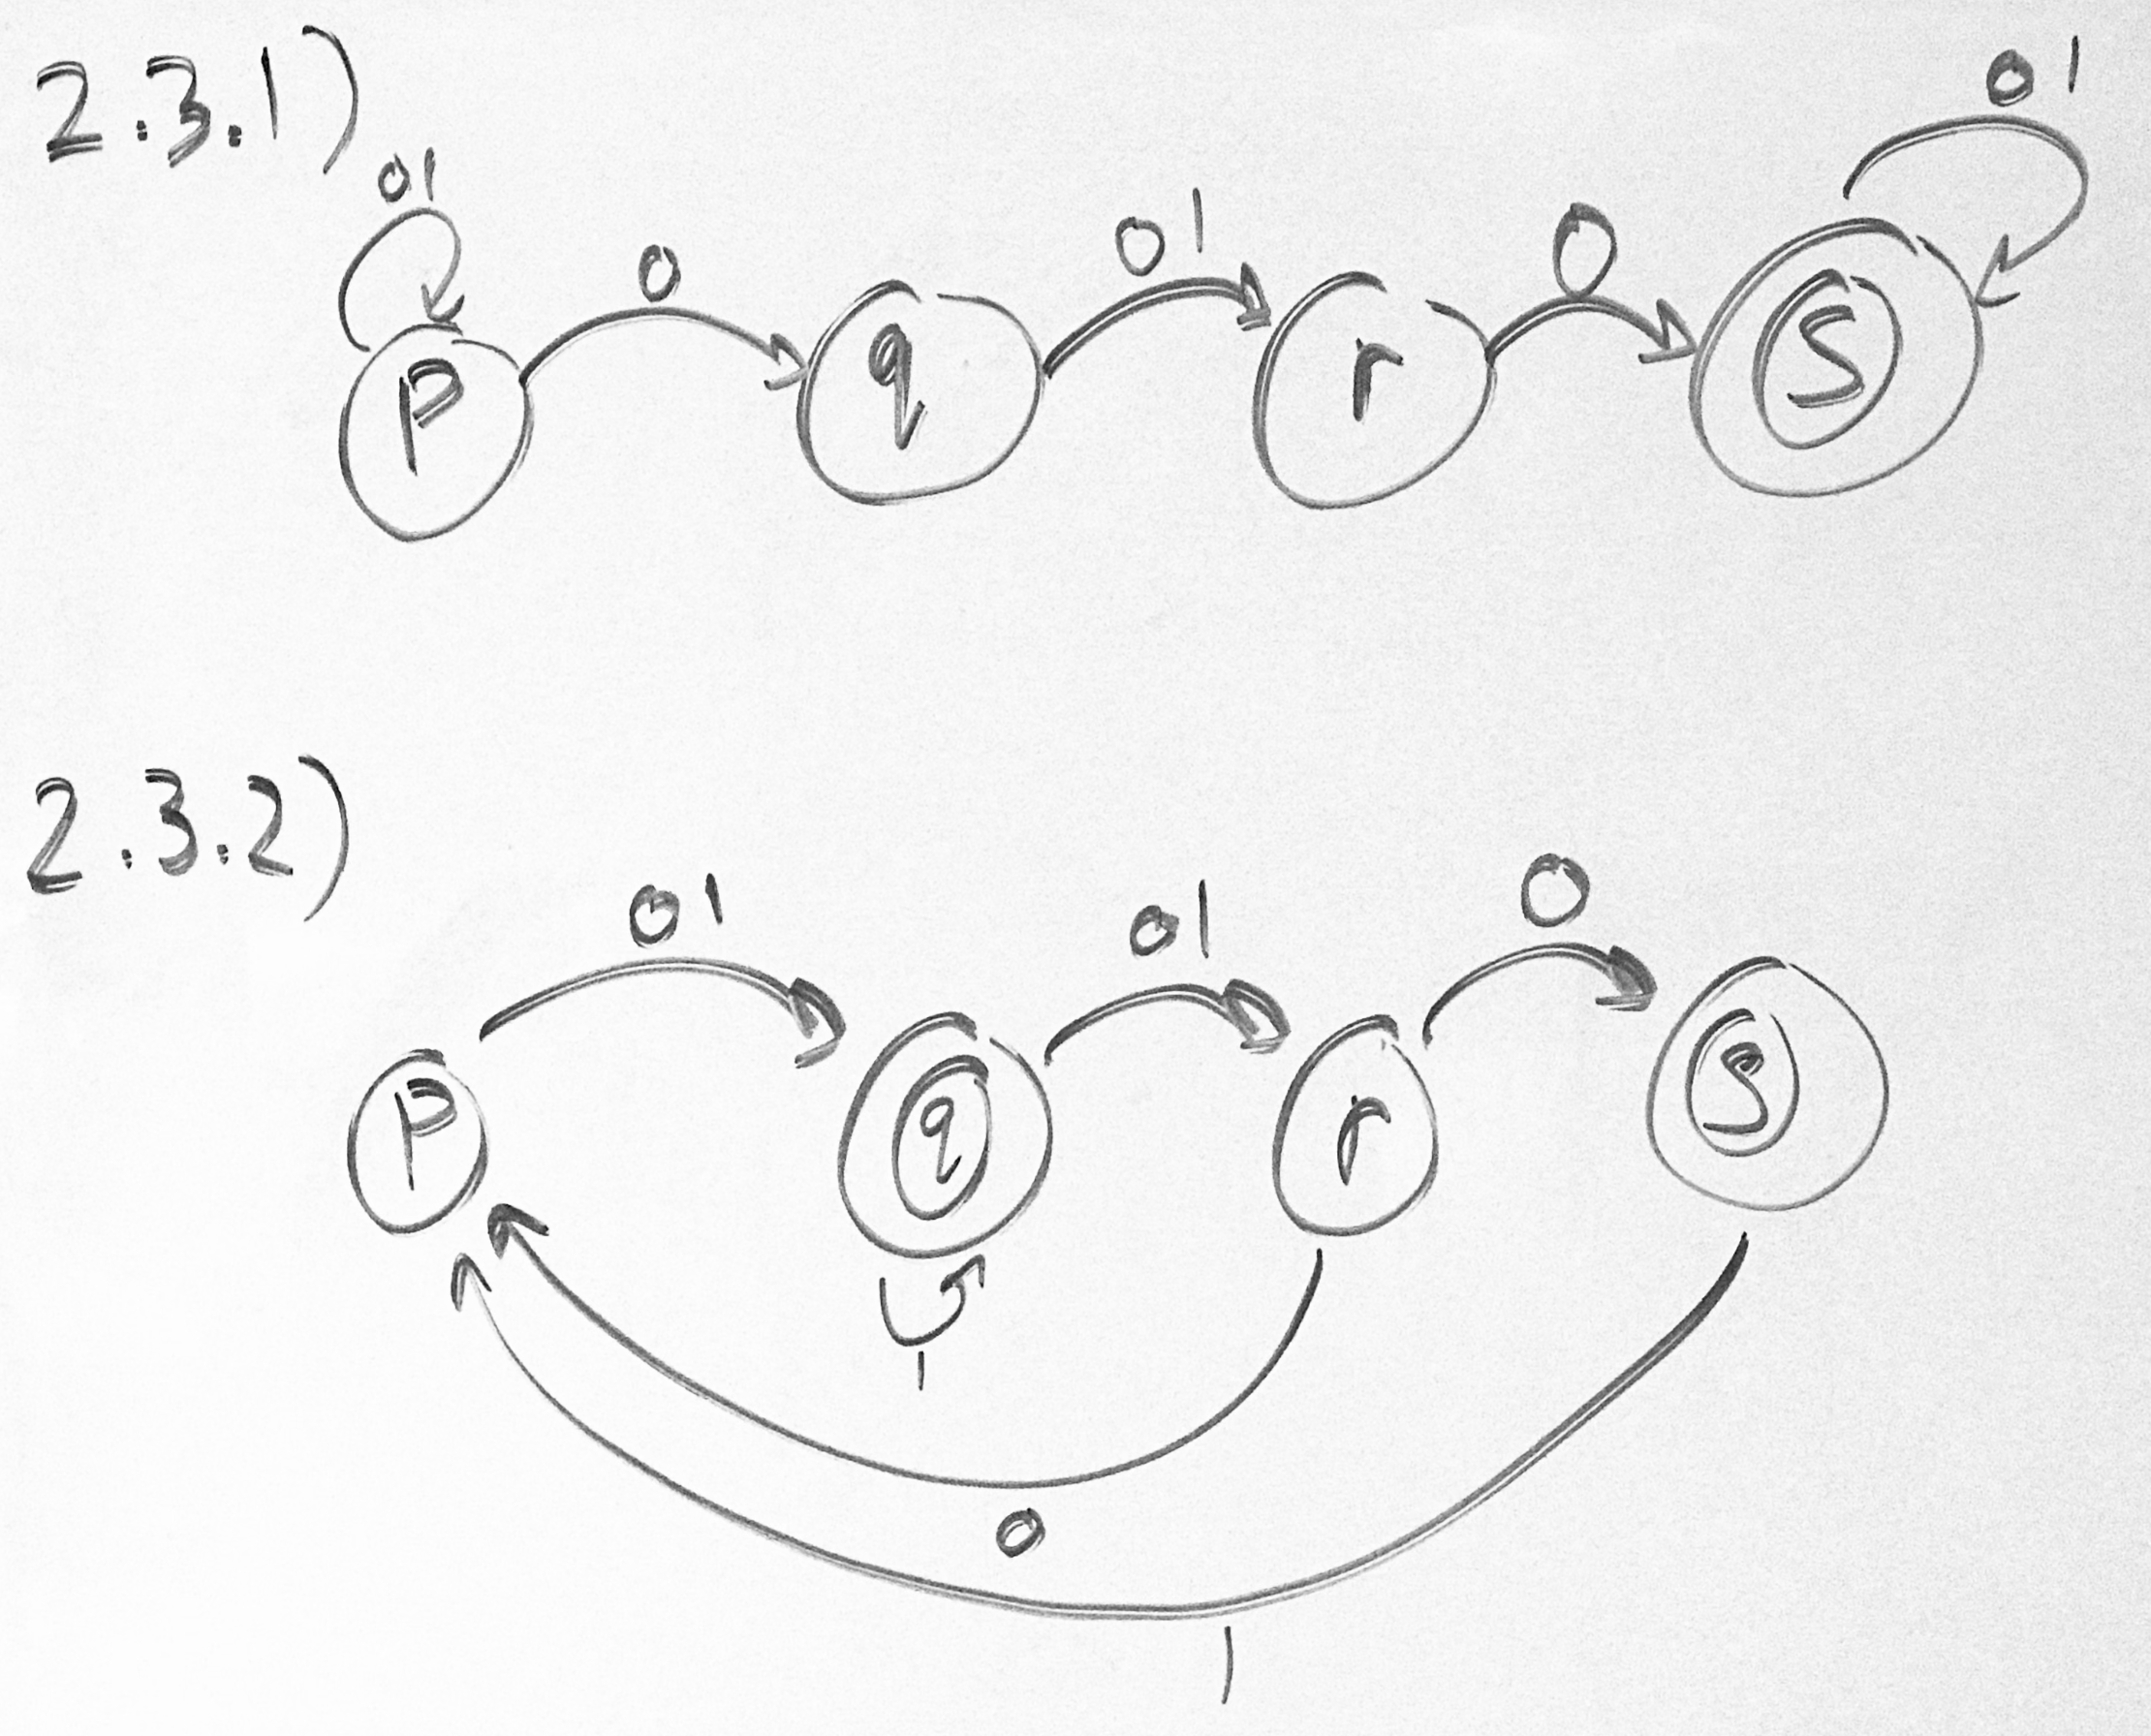
\includegraphics[width=0.50\textwidth]{Images/2.3.1and2.3.2.png}

\medskip\noindent
In order to convert a dfa to an nfa, there can be only one final state. The initial state can remain the same, but the automata must result in one final state every time. Therefore, "final" should not return a set but instead a state.

\begin{lstlisting}[style=HaskellStyle]
  -- convert an NFA to a DFA
  nfa2dfa :: NFA s -> DFA [s]
  nfa2dfa nfa = DFA {
  -- exercise: correct the next three definitions 
  dfa_initial = [nfa_initial nfa],
  dfa_final = let final qs = disjunction (map(nfa_final nfa) qs) in final,
  dfa_delta = let
    f [] c = []
    f (q:qs) c = concat [nfa_delta nfa q c, f qs c] in f }
\end{lstlisting}

\subsection{Week 4}

\medskip\noindent
\begin{lstlisting}[style=CStyle]
  // a fibonacci function showing most features of the C-- language

  int mx () {
    return 5000000 ;
  }

  int main () {
    int lo ; 
    int hi ;
    lo = 1 ;
    hi = lo ;
    printf("%d",lo) ;
    while (hi &lt; mx()) {
      printf("%d",hi) ;
      hi = lo + hi ;
      lo = hi - lo ;
    }
    return 0 ;
  }
\end{lstlisting}

\medskip\noindent
This is the parse tree (concrete syntax tree) for the C$--$ code listed above.

\medskip\noindent
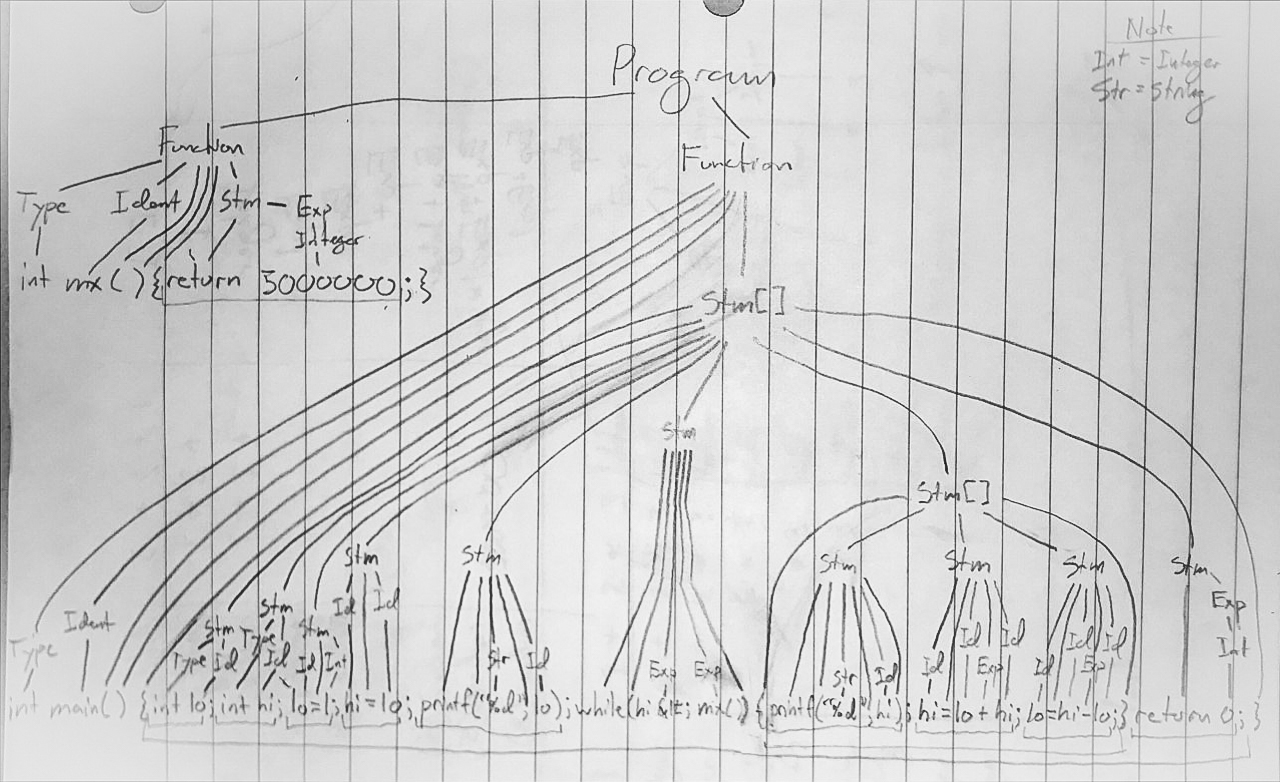
\includegraphics[width=1\textwidth]{Images/ConcreteSyntaxTree.jpg}

\section{Project}
 

\section{Conclusions}\label{conclusions}

\begin{thebibliography}{99}

\end{thebibliography}

\end{document}
